\section{The on-demand evaluation paradigm}
\begin{figure}
  \centering
  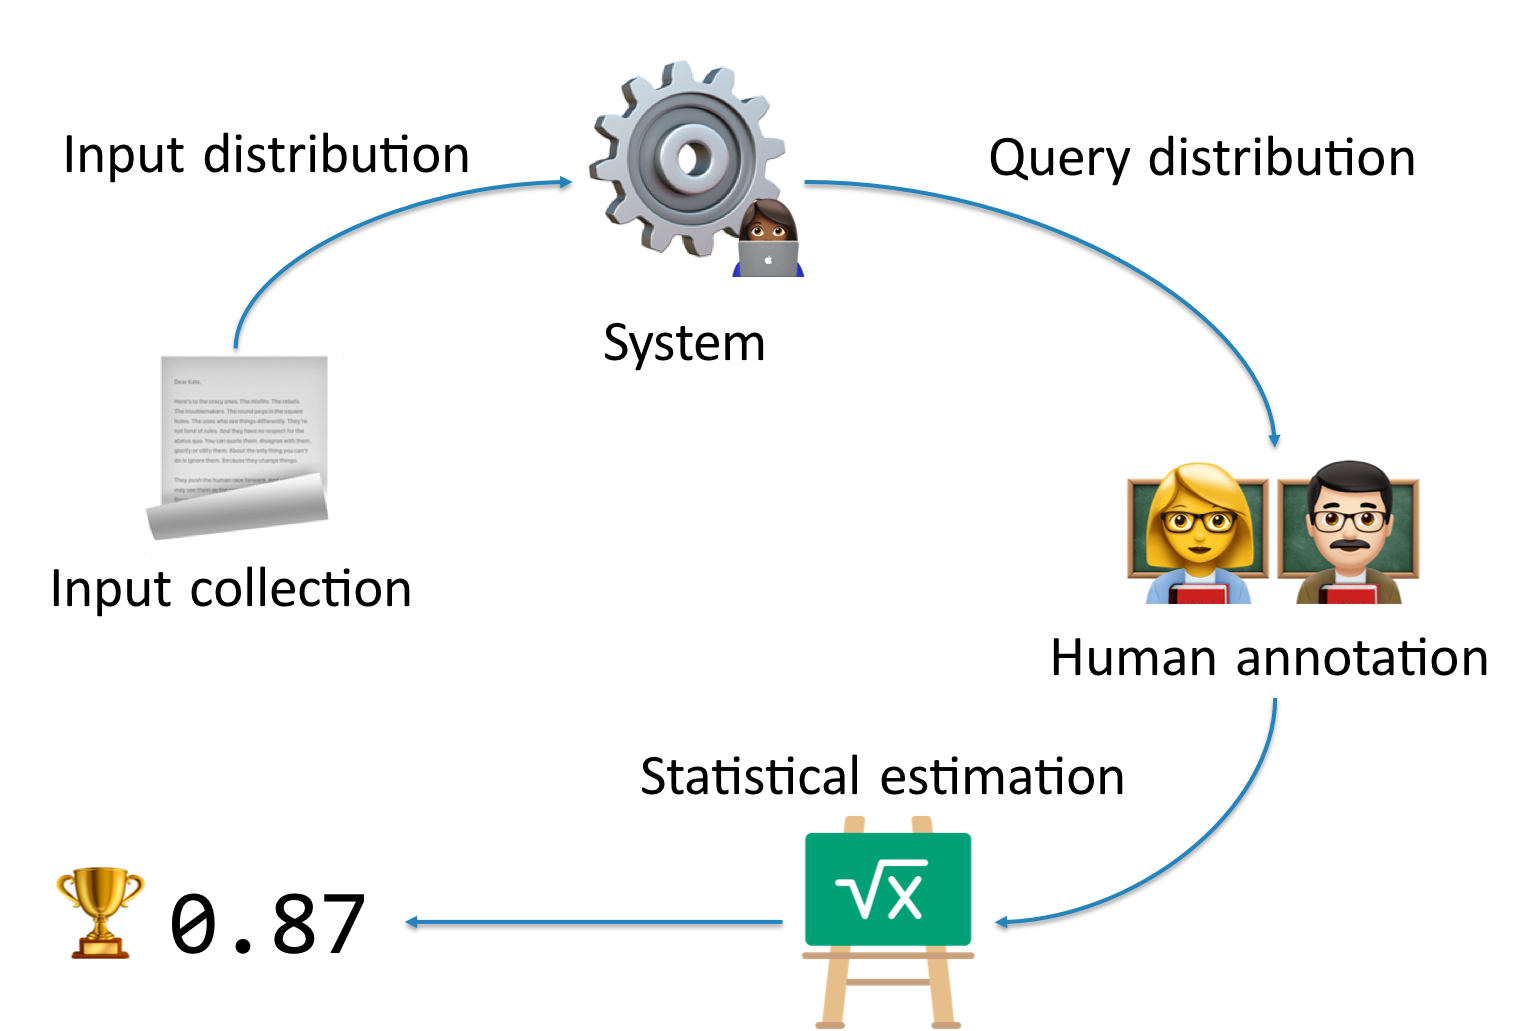
\includegraphics[width=0.6\textwidth]{figures/overview}
  \caption[Overview of the on-demand evaluation paradigm]{\label{fig:conclusions:overview}
  An overview of the on-demand evaluation paradigm. 
  First, we identify a \textit{source of inputs} (e.g.\ documents) or a distribution over the same that are provided to the \textit{system}.
  Next, we specify which inputs to evaluate using a \textit{query distribution}; the query distribution plays the role of a dataset designer by identifying which phenomena we would like to prioritize.
  The linchpin of the paradigm is conducting a \textit{human annotation} as necessary on the system output. 
  Finally, annotations from different systems are combined using a \textit{statistical estimator} to produce a final unbiased evaluation score.
  Additionally, these annotations can be used by system designers to further improve their systems.
  }
\end{figure}

We present on-demand evaluation paradigm as a general evaluation paradigm for \textit{problems where a static test collection would be incomplete}.
The key idea is to overcome the incompleteness of test collection by querying human annotators on-demand.
\reffig{conclusions:overview} presents an overview of the framework: 
First, the evaluation designer decides on an \textit{input source} for the systems being evaluated.
The system then produces output on all of these inputs, but we may not be able to evaluate them because of the incompleteness of the data.
Next, we sample a subset of the system output according to a \textit{query distribution} and collect human annotations for these if they do not already exist.
Finally, the annotations obtained are combined with existing annotations to evaluate and improve the system.

We'll describe the key design decisions and challenges for each of these steps next.

\subsection{Identifying what to annotate}

In static test-collections the dataset designer (e.g., the LDC in the TAC KBP tasks) typically manually identifies input-output pairs that are ``interesting'', because they provide important or challenging use cases for the system.
In contrast, with on-demand evaluation, we get to pick which system predictions we should annotate \textit{at evaluation time}.
Simply annotating a random selection of a system's predictions 

leads to a poor 

This added flexibility allows us to specify 
pick for annotation may depend on the output itself, as  and we will need to specify a sampling distribution to capture exactly these ``interesting'' cases.



Thus, we must \textit{reify} what the goals of our evaluation are and identify specific query distributions that formalize them.
\refchap{kbpo} we saw a couple of examples of these: one query distribution could target performance of the system on particular classes, while another could focus on rare entities.
Unlike in the earlier mode of creating several separate test collections, in \refchap{kbpo} we show how we can use the same set of annotated examples to evaluate many different query distributions using importance-reweighting.

The key challenge when identifying a query distribution is ensuring that it properly reflects our evaluation goal.
Identifying the right query distribution does require some experimentation, but also allows us to draw more precise and statistically significant conclusions.
Given a static query distribution, it is usually straightforward to sample from it.
That said, it is also possible to dynamically update our query distribution during our evaluation.
In \refchap{otj} we used the system's confidence scores to dynamically decide what to annotate.
Unfortunately, an open question is what statistical guarantees we can obtain when dynamically identifying samples.

\subsection{Human annotations}
Once we have identified which examples to annotate, we must query human annotators for their feedback.
The ability to get human annotations on demand is the lynchpin of this new paradigm and is enabled by a host of modern crowdsourcing frameworks like \href{requester.mturk.com}{Amazon Mechanical Turk}, \href{https://www.figure-eight.com/}{Figure Eight} or \href{https://daemo.org}{Daemo}~\citep{gaikwad2015daemo}.
These platforms serve as labor marketplaces where it is easy and quick to hire people to answer questions, label images or text, etc.

\paragraph{Annotation interfaces.}
Having access to human annotators is particularly well suited for our purposes because the underlying difficulty when evaluating tasks such as text summarization, question answering or knowledge base population is human subjectivity.
Put differently, if our end goal is to provide summarize information \textit{for people}, it is fitting that it be judged by people as well.
At the same time, it is often non-trivial to properly communicate the subjective evaluation criteria to a non-expert annotator.
Thus, interface design and instructions are an incredibly important components when crowdsourcing.
The precise interface varies depending on the task and can range from something very simple like a Likert scale survey in \refchap{price} to something significantly more complex like the exhaustive annotation interfaces presented in \refchap{kbpo}.

Depending on the task, it may also be necessary to reformulate what annotations we obtain.
In \refchap{price}, we show that asking people to \textit{edit} a system generated summary and measuring the edit distance results in a more objective metric than simply asking for Likert scale judgments.
When annotating a linguistically nuanced task like semantic role labeling, \citet{he2015question} simplified the annotation schema by using specific questions for roles, e.g., asking ``who finished something'' in order to identify the ``agent''.

\paragraph{Interpretable annotations.}
Another consideration when deciding which annotations to solicit from crowdworkers is whether or not the annotations are \textit{interpretable}.
Interpretable annotations like the edits or highlighting justifications we collected in \refchap{price} not only make it easier to identify systematic annotation errors (which can be resolved e.g.\ by iterating on the instructions) and make the task easier to understand for the crowd worker, but also enable finer grained quantitative error analysis.
As another example, \citet{ling2017teaching} showed how natural language feedback could be used to learn how to caption images better.

\paragraph{Correcting errors in annotations.}
Despite these different approaches to improving the quality of annotations, it is hard to avoid errors made by confused or malicious workers.
Explicit models of the workers and their errors, e.g., ones proposed by \citet{dawid1979maximum}, \citet{passonneau2014benefits} or \citet{branson2017lean}, allow us to aggregate information across multiple workers to correct their errors.
In \refchap{otj}, we showed how we could use a model to dynamically identify when crowdworkers may be confused and used this information to collect additional annotations.
Such models will be necessary when evaluating complex subjective tasks like text summarization.

\subsection{Statistical estimation}
Finally, we must aggregate the human annotations to provide a meaningful quantitative score for a system.
Naively, we can always simply aggregate a suitable metric like precision, accuracy or edit distance using the human annotations, but this will not be economically scalable in the long run.
Thus, a statistical estimator that allows us to \textit{amortize} costs as we evaluate multiple systems \textit{and multiple evaluation metrics} is crucial to making the on-demand evaluation paradigm practical.
The key contribution of this thesis is showing that we can amortize costs with the appropriate statistical estimation techniques.

\paragraph{Precision and recall.}
In \refchap{kbpo}, we proposed efficient estimators for two widely used metrics, \textit{precision} and \textit{recall}.
Computing precision relies entirely on the output generated by a single system, but we showed that by using the annotations from other systems we were able to decrease the variance by a factor of four.

Accurately measuring and improving on \textit{true recall} is vital to being able to develop systems that identify \textit{new} things.
Thus far, most evaluations of open-domain tasks like knowledge base population have only reported \textit{pooled recall}, an approximation that relies on the predictions of a static collection of systems.
We showed that this approach results in a significant and systematic bias that prevents researchers from being able to measure genuine improvements.  
Instead, we leverage the recall calculated on a small, randomly selected collection of documents from the corpus.
Using our statistical estimator, we are able to correct the bias of pooled recall computed on a growing set of systems and thus decrease variance by a factor of almost four.

In both these cases, we have been able to successfully amortize costs over multiple participating systems.
The degree of cost saving really depends on the extent of overlap between systems, is best suited for problems with finite incompleteness.
We believe these techniques should easily transfer to clustering based metrics needed for entity detection and linking and co-reference resolution.

\paragraph{Black-box metrics.}
In \refchap{price}, we execute the on-demand evaluation paradigm in the setting of \textit{infinite incompleteness}, where no two systems are likely to significantly overlap in their predictions.
Of course, as a consequence, system answers also do not overlap with the reference answers in test collections.
The existing solution to this problem is to adopt a \textit{automatic metric} that serves as a similarity function between the system generated answer and reference answer.
Unfortunately, we show that existing automatic metrics not only correlate poorly with human judgment, but are \textit{biased} in that their correlations differ significantly based on the system.

In our work, we have identified an \textit{optimal} estimator to \textit{debias} these automatic metrics.
We prove that the poor correlation also fundamentally lower bounds the number of annotations need to correct the bias;
  in practice, we need almost as many human annotations to correct the bias as to conduct an complete human evaluation!
Thus, in the setting of infinite incompleteness, we have provided optimal estimation techniques, but still haven't been able to successfully amortize costs.

\paragraph{Active learning and dynamic sampling.}
Hypothetically, we could make annotation more efficient if we could dynamically pick which samples to annotate based on the systems performance on previously collected samples.
The key challenge in doing so is correcting for the sampling bias that arises as the distribution over what to sample changes every time we perform an annotation.
Unfortunately, much of the active learning literature focuses only on the generalization performance of a model trained on the samples, and not on unbiased estimation.
The dynamic annotation scheme we proposed in \refchap{otj} is able to evaluate and error-correct systems \textit{at test time}, but does not have access to a query distribution on which to compute an evaluation score.
As such, identifying an efficient, unbiased, dynamic annotation scheme is an important open problem for on-demand evaluation.

\paragraph{Quantitative error analysis.}
Apart from merely obtaining a single quantitative score with which to compare systems, the goal of evaluation is to quantify the limitations of current systems in order to provide direction for future work.
This is often manifested in authors conducting a qualitative error analysis, wherein a small sample of system output is manually inspected and coded for particular language errors.
With humans-in-the-loop, it is possible to collect far more data and conduct a more fine-grained error analysis than was previously possible.

However, by using an appropriate statistical estimator, we can also significantly decrease the costs of conduct fine-grained error analysis by efficiently reusing annotations.
As an example, in \refchap{kbpo} we show how we can accurately analyze the errors made by a knowledge base population system on different relations and entity linking without having to re-annotate any data.

\pl{I found the explanation of this paradigm a bit confusing.
The way I understand things is:
(i) you pick an input distribution (both the domain and how much you care about certain entities as in KBP, etc.); this part is static;
(ii) you collect outputs for these inputs somehow so you can at least train a system (you didn't talk about this, but I guess this is necessary?);
(iii) you run systems on all the inputs;
(iv) you adaptively figure out which input/system predictions to ask humans to annotate (is it annotation or evaluation?) and use statistics to produce meaningful numbers (unbiased, low variance, etc.);
(v) maybe use these annotations back as supervision to systems (you didn't talk about this, but would connect to online learning, which may allow you to connect on-the-job-learning ideas)
}

\pl{In general, I'm not sure I would tout this whole thing so much as a framework,
since at least right now, I don't see a single unified story that applies to all NLP tasks;
I feel like the interesting contributions are in the mechanics how to reduce variance, eliminate bias, etc.
not really in the structural aspects that a framework typically offers
}

\pl{also, you should try to really be careful about what the scope of what you're saying is:
is it AI in general (including vision tasks)? NLP tasks? relation extraction?
some of the wording really suggests something rather specific, but 'on-demand evaluation' is such a general term...
}

